\chapter{Executing Requests}
  \label{chap:execute}

  The virtual \qq{Node::execute()} method is responsible for processing a
  \Request:
  
  \begin{verbatim}
  virtual int execute (Result::Ref &resref,const Request &req);
  \end{verbatim}
  
  \noindent The node is supplied a \qq{Request} object, and it is expected to return a
  \qq{Result} by attaching it to the counted ref passed in as the first
  argument. The return value is called the {\bf result code}: this
  incorporates the depmask of the result, plus several additional flags such
  as \RES{WAIT} and \RES{FAIL} (see below).

  A parent node will generally call the \qq{execute()} methods of its
  children. In the current single-threaded implementation, the entire tree
  is evaluated via nested \qq{execute()} calls. In a multi-threaded or
  distributed implementation, the parent will probably call stub methods in
  the communication layer, which will in turn call \qq{execute()} on the
  child nodes.

  \highlightbox{The \qq{Node::execute()} method is the fulcrum of the entire
  MeqTree kernel. A solid understanding of how it works is vital for both tree
  design and node development, and also beneficial to advanced users that need
  to deal directly with trees.}

  
\section{Node::execute() steps}
   \label{sec:execute}
  
  
  The \qq{Node::execute()} method looks at the request, and calls a number
  of virtual {\em handler} methods for various aspects of processing. Most
  node classes will override one or more of these handler method(s) to
  implement their specific node behaviour. \qq{Node::execute()} also
  provides fundamental node functionality, such as cache management and
  exception handling.\footnote{You may have noted that \qq{execute()} is
  declared virtual. Most node classes will only redefine specific handler
  methods, not \qq{execute()} itself.  The possibility to reimplement
  \qq{execute()} is reserved for the exotic cases. This is not to be
  undertaken lightly, however, as the base \qq{Node::execute()} provides so
  much useful behaviour.}

  The base \qq{Node::execute()} performs a number of processing steps. These
  will now be described in detail, grouped by function.
  

\newcounter{execstep}
\setcounter{execstep}{0}
\newcommand{\ExecStepBox}[2]{\highlightbox{\mbox{\bf #1. } #2}}
\newcommand{\ExecStep}[1]
{\addtocounter{execstep}{1}\ExecStepBox{Step \arabic{execstep}}{#1}}
  
\subsection{Checking the cache}

  \ExecStepBox{Init return code}{Set the current return code to 0. It will be
  accumulated in further steps via a bitwise-OR operation.}

  \ExecStep{Compare the request id to the previous rqid, if any. Set a local
  ``new request'' flag for the benefit of further logic below.}

  \ExecStep{If there's a cached \Result, and the request id matches the
  cached rqid/depmask (see \ref{sec:cache} for a discussion), immediately
  return the cached \Result\ and cached result code. On mismatch, clear the
  cache and proceed.}
  
  Note that the caching policy also determines how fail-results are dealt with.
  If the cache contains a fail-result, the node may choose to ignore it and
  attempt to recalculate the result to see if the fail conditions have gone
  away.

  \ExecStep{For new requests only: call the virtual \qq{readyForRequest()}
  handler, and if the return value of that is \qq{false}, immediately
  return the code \RES{WAIT} (result will be empty).}
  
\begin{verbatim}  
  virtual bool readyForRequest (const Request &req);
\end{verbatim}

  \noindent The handler is passed the current \Request, i.e., the \qq{req}
  argument to \qq{execute()} itself. The purpose of this handler is to
  support nodes that block on external events. None as such have been
  implemented, so this is currently just a placeholder. The default handler
  always returns \qq{true}.

  \medskip \ExecStep{For new requests only: if a rider subrecord is present,
  parse it and call the virtual \qq{processCommands()} handler to process
  commands targeted at the node (see details in~\ref{sec:CSR}).}

\subsection{Polling children}
    
  \ExecStep{If node has children, call the virtual \qq{pollChildren()}
    handler to pass the request on to the children and collect their
    results. Bitwise-OR the return value of \qq{pollChildren()} into the current
    return code.}

  \begin{verbatim}    
  virtual int pollChildren (std::vector<Result::Ref> &child_results,
                            Result::Ref &resref,
                            const Request &req);
  \end{verbatim}
    
  \noindent The handler is called with the same \qq{resref} and \qq{req}
  arguments that were given to \qq{execute()} itself. Child results should be
  returned via the \qq{child\_results}, which is pre-sized to the number of
  children prior to calling \qq{pollChildren()}.

  The default implementation of \qq{pollChildren()} is appropriate for most
  node classes that pass their requests on to the children unmodified. 
  ``Control'' nodes (e.g. \qq{Sink}, \qq{Solver}, \qq{ModRes}, \qq{ReqSeq}) will
  define their own version. This is the default \qq{Node::pollChildren()}
  behaviour:

  \begin{itemize}

  \item Calls \qq{execute()} (with \qq{req}) on all the child nodes, collects
  their \Result{}s (by ref) into the \qq{child\_results} vector, and
  accumulates a return code as a bitwise-OR of the children's \qq{execute()}
  return values. Note that the refs to child \Result{}s are expected to
  be read-only. 

  \item If the accumulated return code has the \RES{FAIL} bit set, its is
  assumed that at least one of the children has returned a fail-result
  (see~\ref{sec:fail}). In this case, \qq{pollChildren()} creates a new
  fail-\Result\ object, attaches it to \qq{resref}, and fills it with 
  all the fail-records found in child results.

  \item The accumulated return code is the return value of the handler.

  \end{itemize}
  
  Note that \qq{resref} is passed to \qq{pollChildren()} only as a means of
  reporting possible fails. If the handler returns a code with \RES{FAIL} in
  it, it should attach a fail-result to \qq{resref}. If no \RES{FAIL} is
  reported, the handler should leave \qq{resref} alone (in fact, anything it
  does to it will be simply ignored when no \RES{FAIL} is returned.)

  If the \qq{pollChildren()} return value contains \RES{WAIT} or \RES{FAIL},
  \qq{execute()} returns (see section~\ref{sec:execute-return}). Otherwise,
  it proceeds to the next step:

  \ExecStep{If auto-resampling is enabled (see \ref{sec:resampling}), compare
  the resolutions of the child results, figure out a common resolution
  (\qq{Cells}) to resample them to, and perform the resampling. Throw an
  exception if this is not possible.}
  
  Note that if the child results do not contain any \VellSet{}s (which will be
  the case when the \Request\ does not have a \qq{cells} command), this step is
  skipped.
  
  A result \Cells\ may be initialized based on how the resampling went (see
  \ref{sec:resampling}). 

\subsection{Evaluating \qq{cells}}

  \ExecStep{If the request contains a \qq{cells} command (with a \Cells\
  object), call the virtual \qq{getResult()} handler to process the command,
  passing in the vector of child \Result{}s returned by \qq{pollChildren()}.
  The return value of \qq{getResult()}, along with the node's current depmask
  (see~\ref{sec:depmask-node}), is bitwise-ORed into the current return code.}
  
\begin{verbatim}
  virtual int getResult (Result::Ref &resref,
                         const Cells::Ref &cells,
                         const std::vector<Result::Ref> &child_results,
                         const Request &req,bool newreq);
\end{verbatim}
  
  The \qq{resref} and \qq{req} arguments are the same as those passed to
  \qq{execute()}. The \qq{cells} argument is a ref to the result cells, if any
  were initialized during the resampling stage above, or otherwise to the
  \Cells\ in the request (see~\ref{sec:resampling} for details). The
  \qq{child\_results} vector is built up in \qq{pollChildren()}, it will be
  empty if the node has no children. Finally, the \qq{newreq} flag indicates if
  it is a new request, this flag is set in Step~1 above.
  
  The \qq{getResult()} handler is responsible for attaching a \Result\ object
  to \qq{resref}. In most cases, it will create a new object. Note, however,
  that certain nodes may pass on child results transparently (e.g.,
  \qq{ModRes}, \qq{ReqSeq}), they do this by simply copying a ref from the
  \qq{child\_results} vector. 
  
  If \qq{getResult()} returns a \RES{WAIT} code, it is allowed (and expected)
  to leave \qq{resref} unattached. Otherwise, a valid \Result\ must be
  provided! Any errors occurring inside \qq{getResult()} can be reported by
  throwing an exception.

\subsection{Handling exceptions}

  \ExecStepBox{Error handling}{If an exception is thrown at any stage of the
  process, \qq{execute()} will catch it, create an output \Result\ with a
  fail-result describing the exception, and add return the current return code,
  with a \RES{FAIL} flag added in.}

  Thus, throwing an exception is the normal way for \qq{processCommands()},
  \qq{getResult()}, or any other handler to indicate a failure. Note that a
  node should remain in a usable state (i.e. should be able to process further
  \Request{}s) after most exceptions; methods that are liable to leave the node
  in a non-usable state should provide their own exception handling code that
  performs the necessary cleanups and re-throws the exceptions. See the
  \qq{setState()} rollback mechanism described in section
  \ref{sec:state-rollback} for one such example.

\subsection{Caching and returning a \Result}
\label{sec:execute-return}
 
  \ExecStepBox{Returning}{Whenever any kind of \Result\ is returned, it is
  stored in the cache according to the current policy, and returned via the
  \qq{resref} argument. The accumulated return code is returned along with the
  result. If the result is new (i.e. not returned from cache at step 2), the
  \RES{UPDATED} flag is added to the return value.}

  Note that if the accumulated return code contains \RES{WAIT}, then no
  \Result\ is expected (\qq{resref} remains unattached). In all other cases, a
  valid \Result\ object should be attached to \qq{resref} (in case of
  exceptions, this will be a fail-result).

\subsection{All Results are read-only!}

  Prior to returning a \Result, \qq{execute()} recursively changes \qq{resref}
  and all other refs found inside the result object to read-only. This implies
  that the caller of \qq{execute()} (i.e. the parent node, or \qq{MeqServer})
  cannot [legally] change the \Result\ contents. This is deliberate -- the node
  can now hold a ref to the \Result\ in the cache, and be assured that no-one
  can [legally] change the contents. 
  
  In most cases, parent nodes will process the \Result{}s of their children as
  read-only, and discard them afterwards (actually, only the parents' refs are
  discarded -- the \Result\ objects themselves persist if still referenced
  somewhere, e.g., in a child's cache). Some nodes may want to modify child
  \Result{}s ``in place''. To do this, they will need to privatize their refs
  for writing first (see \ref{sec:countedrefs}), thus ensuring that a private
  copy is made if the same object is still referenced somewhere. The same
  applies to individual components of the \Result{}s. Essentially, this is a
  robust copy-on-write mechanism that assures that data is duplicated only when
  needed, with very little effort required from the node developer.
  
  Note also that when a \Result\ is moved across to the scripting layer, some
  sort of copying is implicitly performed. Glish does not deal with \Result\
  objects directly, but rather with their Glish representations.

\section{Result codes}
\label{sec:execute-resultcode}

  As described above, the return value of \qq{execute()} is simply the
  accumulated result code. The result code describes certain properties of the
  returned \Result. Part of it is simply the result depmask (see
  \ref{sec:depmask-result}, the other part contains a number of bitflags listed
  below. Note that the property semantics are defined in such a way that, in
  most practical cases, a flagged property in any child result is inherited by
  the parent's result. This allows \qq{execute()} to accumulate the correct
  result code via a simple bitwise-OR. The following additional flags are
  defined:
 
  \begin{description}
  
  \item[\RES{UPDATED}:] result has changed from that of previous \Request. This
    bit is usually cleared when the node returns a result  from the cache, and
    set otherwise.

  \item[\RES{VOLATILE}:] result may change in response to external events,
    even without new requests. {\em (This is not implemented for now, and only meant
    as a placeholder for future developments, such as dynamically growing
    domains, partial integration, etc.)}

  \item[\RES{FAIL}:] result is a fail. Note that this is not the same thing as
    a result containing some mix of valid and failed VellSets; rather, this
    indicates a failure for the whole result overall. \RES{FAIL}s are usually
    generated in an exception handler. Note that the default implementation of
    \qq{pollChildren()} and \qq{execute()} causes fails to cascade down the
    tree.

    When this flag is returned, a \Result\ object is still expected; it should
    contain one or more fails describing the error. Note that depmasks can be
    meaningfully combined with \RES{FAIL}, to indicate that the fail depends on
    something (i.e. may go away if a particular dependency changes). The
    ``smart'' caching policy may make use of this. 

  \item[\RES{WAIT}:] no result available, wait for notification or try later.
    If this flag is raised, then no \Result\ should be returned. Note that
    dependency flags can be meaningfully combined with \RES{WAIT}, since it
    usually possible to indicate the dependencies of a node in advance. No
    current code uses this, however.

  \end{description}
  
  The return value of a node's \qq{getResult()} method should describe any {\bf
  additional} properties introduced by the \qq{getResult()} calculation
  (additional with respect to the node's current depmask -- see
  \ref{sec:depmask-node}). Most function nodes will return zero, indicating
  no additional dependencies.

\section{Commands in request riders}
  \label{sec:rider}
  \label{sec:CSR}
  \label{sec:rider-setstate}

  The optional \qq{rider} sub-record of a \Request\ is used to send commands to
  nodes. The \qq{Solver} node, for example, relies on this feature to send up
  parameter updates during iterative solutions. Commands are specified as sets.
  Each {\bf command set} is a record (\qq{DataRecord} in C++), with the field
  names (i.e. HIIDs) being the commands per se, and the field value being the
  command value a.k.a. arguments. Commands with no arguments are indicated with
  a boolean \qq{true}, a boolean \qq{false} value implies that the command is
  {\bf not} issued.\footnote{This may seem redundant -- why not simply omit a
  command if it is not meant to be issued? Consider though that Glish has no
  built-in facility for {\em removing} record fields. The ``false=no command''
  convention allows one to effectively remove a command from an existing set by
  assigning the \qq{F} value to it.} If the set contains multiple commands,
  they are processed in a specific order determined by the node class. Some
  example commands are:

  \begin{description}
  
  \item[\qq{state}:] changes the state of a node (available for all nodes);
  
  \item[\qq{add\_dep\_mask}:] adds symdep masks (available for all nodes,
  discussed in \ref{sec:symdeps}).

  \item[\qq{update\_values}:] incremental updates of solvable parameters (see
  documentation for the \qq{Solver} and \qq{Parm} nodes).
  
  \end{description}
  
  Since commands are seen as record fields in Glish, and plain HIIDs in C++, we
  will use both forms (\qq{foo\_bar} and \qq{"Foo.Bar"}) interchangably.
  
\subsection{The command handler}

  Commands are processed by a virtual handler method, called from
  \qq{execute()}:

\begin{verbatim}
  virtual void processCommands (const DataRecord &rec,Request::Ref &reqref);
\end{verbatim}

  The \qq{rec} argument is the command set to be processed (see below). The
  \qq{reqref} argument is a ref to the current \Request. Because the
  \qq{processCommands()} handler is called before \qq{pollChildren()}, it can
  modify the request (i.e., add commands to it) before it is passed on to the
  children. \qq{Node} itself, for example, uses this capability when
  accumulating symdep masks (see \ref{sec:symdeps}). The \qq{reqref} should be
  privatized for writing before a \Request\ is modified, because requests are
  normally passed around as read-only.

  Node classes implementing their own commands will need to redefine this
  handler. It is important, however, that the new handler calls the parent
  class's handler first, so that commands implemented in superclasses
  (especially \qq{Node} itself) are handled properly. Unknown commands should
  be ignored -- in fact, handlers are usually implemented to simply look up
  known commands, and ignore the rest.
  
  Any errors arising during command processing may be indicated by throwing
  exceptions (these will be caught by \qq{execute()}). The handler should take
  care to perform any cleanup, and leave the node in a usable state.

  The base handler, \qq{Node::processCommands()}, processes all standard
  \qq{Node}-level commands. These are listed in section
  \ref{sec:commands-Node}.

\subsection{Rider subrecord layout}
  
  The rider record is structured so that it is possible to associate a command
  set with a specific node or a set of nodes. Each node thus checks if the
  request contains any commands for itself. Note that in a very large tree,
  such repeated checks may grow quite expensive. For this reason, nodes that
  need to receive a lot of commands should be assigned to a {\em node group}. 

  A node may be associated with one or more groups. Each group is identified by
  a \qq{HIID}, a node's group assignments are a part of its dynamic state (see
  \ref{sec:state-Node}). All nodes implicitly belong to the \qq{all} group. A
  node's groups are used as a first-level index into the \qq{rider} record. If
  a node belongs to groups \qq{foo} and \qq{bar}, then \qq{Node::execute()}
  will check for the {\em command subrecords}\/ ({\bf CSR}s) \qq{rider.foo},
  \qq{rider.bar}, and \qq{rider.all}, in that order, and process any CSRs that
  it finds.

  Judicious use of node groups practically eliminates the overhead of command
  lookup. The rider itself contains very few fields (if any), so looking up the
  CSR for a group is very fast. If your tree frequently uses commands to
  control a small subset of nodes (e.g., a solve-tree uses commands to update
  solvable parameters), these nodes should be placed in a group of their own,
  and commands should be kept in that group's CSR. All other nodes will only
  check for the \qq{all} CSR -- which is usually not present. Thus, only the
  required subset of nodes will engage in the possibly expensive business of
  CSR parsing and command processing.
  
  The \qq{all} CSR allows for commands to be sent to any node; but because of
  the associated overhead, this should only be used for infrequent operations
  (e.g., reconfiguring a tree -- as opposed to iterative solving).

\subsubsection{CSR layout}
  
  Each CSR contains a number of command sets. These command sets may be
  associated with specific nodes. There are three ways to specify these
  associations (we will use \qq{csr} here to refer to the CSR itself):

  \paragraph{All nodes in group:} The command set contained in the field
  \qq{csr.command\_all} applies to all nodes in the group. For example:

\begin{verbatim}
  - req.rider.foo.command_all
  [ save_polc=T,state=[solvable=F] ]  
\end{verbatim}

  ...will call \qq{processCommands()} on all nodes in group \qq{foo}, with the
  command set \qq{[save\_polc=T,state=[solvable=F]} (meaning save polcs, and set
  to non-solvable).

  \paragraph{Via node index:} Command sets may be associated with a node index.
  This is done via \qq{csr.command\_by\_nodeindex}, which is essentially
  a map from node index to command set. For example:

\begin{verbatim}
  - req.rider.foo.command_by_nodeindex
  [ #19 = [ value=1,save_polc=T ], #41 = [ value=2,save_polc=T ] ]
\end{verbatim}

  ...will cause a \qq{processCommands()} call on nodes 19 and 41, but only if
  these nodes actually belong to group \qq{foo}. (Note that since Glish only
  supports strings for record field names, the \qq{'\#{\sl ddd}'} form is used
  to specify a ``numeric'' node index.)

  \paragraph{Via lists:} The third way is to associate command sets with  lists
  of nodes matched by name or node index. This is done via a list of records
  in \qq{csr.command\_by\_list}. For example:

\begin{verbatim}
  - req.rider.foo.command_by_list
  [ #1 = [ name="RA DEC",nodeindex=[17,32],
           command=[ save_polc=T,state=[solvable=F] ] 
         ],  
    #2 = [ command=[ state=[solvable=F] ] ] 
  ]
\end{verbatim}

  ...will call \qq{processCommands()} with the first command set on nodes `RA',
  `DEC', 17 and 32 (if they belong to group \qq{foo}), and with the second
  command set on all other nodes in group \qq{foo}. To be more specific, the
  \qq{command\_by\_list} field is treated as a list of records. Each record in
  the list must contain a \qq{command} field (the command set itself),  plus an
  optional \qq{name} field (string or list of strings) and/or an optional
  \qq{nodeindex} field (integer or list of integers). \qq{Node::execute()} will
  iterate through the list of records one by one; if the node's name is found
  in \qq{name}\footnote{In the future, pattern matching will be supported as
  well.}, or the node index is found in \qq{nodeindex}, then
  \qq{processCommands()} is called with the contents of \qq{command}. Once a
  match is found, list processing stops. As a special case, if neither
  \qq{name} nor \qq{index} is specified, then the entry is a ``wildcard''
  matching any node. Wilcards are only useful at the end of the list, to catch
  nodes not matched by previous entries.

\subsection{Command evaluation order}

  As you can see, the rider allowss for more than one command set per node. In
  this case, \qq{processCommands()} will be called several times, once for each
  set. It is important then to define the order in which the rider is parsed:

  \begin{itemize}
  
  \item The outer loop is over node groups, in the order in which they are
  specified in the node's state record. The \qq{all} group is checked last.

  \item Within a group's CSR, the processing order is from least specific to
  most specific: \qq{command\_all}, \qq{command\_by\_list},
  \qq{command\_by\_nodeindex}.

  \item Once a command set is passed to a node's \qq{processCommands()} method,
  the order of processing is determined by the node class implementation.
  Generally, a subclass should call its parent's \qq{processCommands()} first,
  so general commands (such as \qq{state}) will be processed before more
  class-specific commands (such as \qq{save\_polc}).

  \end{itemize}
  
\subsection{Standard node commands}
\label{sec:commands-Node}

  The following is a list of standard commands implemented at the \qq{Node}
  level. Commands are listed in the form of Glish record field names. 
  The actual order of processing is the same one as given here:
  
  \begin{description}
  
  \item[resolve\_children:] resolves all children specified by name into actual
  nodes. An exception is thrown if a name does not match any known node. This
  command is normally issued by \qq{MeqServer} at initialization time, in
  responce to a \qq{"Resolve.Children"} request. This command has no value.
  
  \item[state:] calls \qq{setState()} (see \ref{sec:setState}) with the command
   value. This command thus allows for any field of the dynamic state to be
   modified.
   
  \item[clear\_dep\_mask:] clears accumulated symdep masks (see
  \ref{sec:symdeps}). This command has no value.
  
  \item[add\_dep\_mask:] accumulates symdep masks (see \ref{sec:symdeps}). The
  command value is a record of symdep:mask pairs.

  \item[init\_dep\_mask:] if the node is a dependency generator (see
  \ref{sec:symdeps}), this command causes it to add its generated symdep
  masks to the request, as an \qq{add\_dep\_mask} command placed into
  the \qq{command\_all} field of the CSR for the configured gendep group.
  
  \end{description}

\subsection{Building up command riders in Glish}

  In Glish, the command rider is simply a part of the \qq{request} record, and
  may be created and manipulated just like any other [sub]record. In addition,
  \qq{meq/meqtypes.g} defines some handy shortcuts for adding commands to a
  request:
  
  \begin{verbatim}
  const meq.add_command := function (ref req,group,node,command,value=T);
  \end{verbatim}

  This function modifies the request object passed in via the \qq{req}
  argument. A CSR for \qq{group} will be initialized if required, and a
  \qq{command} with the specified \qq{value} added to the appropriate field of
  the CSR. The \qq{node} argument specifies the target node(s) as follows:

  \begin{itemize}  
  
  \item an empty list (i.e. \qq{[]}) targets command at all nodes. The command
  is added to the \qq{command\_all} set.
  
  \item a single integer is treated as a node index. The command is added
  to \qq{command\_by\_nodeindex} (initializing a command set if necessary).
  
  \item a list of integers is treated as node indices. The command is added to
  \qq{command\_by\_list}, with a \qq{nodeindex} key.
  
  \item a string or a list of strings is treated as node name(s).The command is
  added to \qq{command\_by\_list}, with a \qq{name} key. 
  
  \item an empty string array (\qq{""}) adds a wildcard entry to
  \qq{command\_by\_list}.

  \end{itemize}
  
  A second shortcut is handy for inserting a state update command:

  \begin{verbatim}
  const meq.add_state := function (ref req,group,node,state);
  \end{verbatim}
  
  This will add a \qq{state} command, with the supplied \qq{state} record as its
  value. All other arguments have the same meaning as for \qq{add\_command()}.

\section{Resolution \& resampling}
\label{sec:resampling}

  Resolution \& gridding is a complicated business. Most nodes expect their
  children's results to have the same resolution (i.e. same \qq{Cells}), yet
  performance constraints require our trees to operate at different
  resolutions. \qq{Node} implements a flexible mechanism for automatically
  controlling the resolution of child results. Before going into detail, it
  helps to take a step back and review some basic requirements:

  \begin{itemize}
  
  \item In the first instance, the grid/resolution is determined by incoming
  data. We'll call this the {\bf full resolution} grid.

  \item It may be prohibitively expensive to evaluate some subtrees (e.g.
  predict) at full resolution. Thus we should support going from full
  resolution to {\bf reduced resolution} ({\bf integration}) and back ({\bf
  upsampling}). 

  \item Parent nodes will not always have sufficient information to determine
  what the best resolution for a child is (i.e. the optimum predict resolution
  may perhaps be only determinable within the predict subtree). Thus, a child
  should be able to  return data at any resolution is deems fit, and let the
  parent deal with it.

  \end{itemize}


\subsection{Treatment of resolution}
  
  To satisfy these requirements, the following behaviour w.r.t. resolution
  is implemented:
  
  \begin{enumerate}
  
  \item The {\bf requested resolution} (or grid) is defined by the \Cells\
  object supplied with the \qq{cells} command of a \Request.

  \item The requested resolution is merely a hint! A node is not obligated to
  honor the grid of the \Cells. It must, however, honor the envelope domain.
  The gridding of the result is indicated by the \Cells\ returned in the
  \Result\ object.
  
  \item Some leaf nodes (e.g. \qq{Const} and \qq{Parm} with no time-frequency
  dependence, when configured to return samplings and not integrations) return
  resolution-free \Result{}s. This is indicated by a missing \Cells\ in the
  \Result. 

  \item Other leaf nodes (e.g. \qq{Parm}, \qq{Freq}, \qq{Time} -- generally,
  nodes meant to evaluate some analytic function over the domain) are easily
  able to evaluate themselves over any given grid. These nodes will always
  return a \Result\ at the requested resolution; the tree designer may rely on
  this behaviour as it is part of the contract for those nodes.

  \item Data-driven leaf nodes (e.g. \qq{Spigot}) completely ignore the
  requested resolution. The gridding of their \Result\ is fully determined by
  the layout of incoming data.

  \item Most non-leaf nodes with multiple children (e.g., most of the
  \qq{Function}-derived nodes) can only operate on child results of the same
  resolution. In the event that different resolutions are returned, any node
  can be configured to {\bf auto-resample} child results to a common
  resolution. This is done by \qq{Node::execute()} prior to calling
  \qq{getResult()}.

  \item Some special nodes (such as \qq{ModRes}) can modify the resolution in
  the request before passing it up.
  
  \end{enumerate}
  
  Note each node's treatment of the requested resolution (i.e.
  honor/ignore/modify) is part of the node class contract, and should be
  clearly documented in the Node Reference. Thus, while parent nodes have no
  control over (or knowledge of) what resolution their children are going to
  use for their results, the tree designer can always see the global picture,
  and determine which resolution is used where in the tree. By enabling
  auto-resampling at key points in the tree, and possibly adding some
  \qq{ModRes} nodes, the designer can always ensure predictable results.
  
  The brute-force approach (as opposed to careful tree design) is to enable
  auto-resampling at all nodes. This, however, is a waste of CPU, and is never
  actually necessary.

\subsection{Selecting auto-resampling modes}

  Auto-resampling is enabled via the node state record, on a node-by-node
  basis. The actual resampling is performed in \qq{Node::execute()}, and it can
  follow one of several strategies:

  \begin{description}
  
  \item[Upsample:] Find the highest resolution among child results, upsample
    all other results to it.

  \item[Integrate:] Find the lowest resolution among child results, integrate
    all other results to it.

  \item[Use Resolution Driver:] Resample everything to the resolution of a
    specific child (this child is called the {\em resolution driver}\/).

  \item[Use Request:] Resample everything to the resolution of the \Request. If
    this strategy is selected, the node is guaranteed to honor the requested
    resolution. If all child results have the same resolution, but it is
    different from the requested one, resampling is performed.

  \item[Fail:] Fail outright (return a fail-result, that is) if resolutions
    differ. This option is mainly useful for debugging; in a properly designed
    tree, any node that can potentially encounter this situation should be
    configured to use one of the other strategies.

  \end{description}
  
  Note that when selecting a high or low resolution for integration or
  upsampling, resolution-free results are ignored, since they never require
  resampling.

  The auto-resampling strategy is determined by two fields in the node state
  record (note that this is dynamic state). The \qq{resample\_child\_index}
  field enables the ``Use Resolution Driver'' strategy, if set to an ordinal
  child number ($\ge 1$ in Glish, $\ge 0$ in C++ -- note the \qq{index} suffix
  and remember automatic 0-1-base conversion discussed in section
  \ref{sec:01base}) or a \qq{HIID} child label (see \ref{sec:children}). The
  specified child becomes the resolution driver. If the field is set to boolean
  \qq{false}, or an out-of-bounds number ($<1$ in Glish, $<0$ in C++), then
  this resampling strategy is not enabled.

  If the resolution driver returns a resolution-free result (see
  \ref{sec:result-empty-cells}), then a fail is reported. This situtation
  indicates an error in tree design, since resolution-free results are returned
  by only a few nodes, under well-defined circumstances.
  
  If a resolution driver is not enabled, then the \qq{auto\_resample} field can
  define another resampling strategy. It can be set to one of the following
  values:

  \begin{description}

  \item[NONE $(=0)$:] do nothing, do not even check the child resolutions. This
  is the default setting initialized by the \qq{Node} class constructor. 

  \item[FAIL $(=-2)$:] check resolutions and return a fail-result if they do
  not match. This is the default setting initialized by the \qq{Function} class
  constructor. Since this is somewhat slower that the \qq{NONE} setting, the
  default for optimized builds may possibly be changed to \qq{NONE} in the
  future.

  \item[INTEGRATE $(=-1)$:] select the ``Integrate'' strategy.

  \item[UPSAMPLE $(=1)$:] select the ``Upsample'' strategy.

  \item[REQUEST $(=2)$:] select the ``Use Request'' strategy.

  \end{description}
  
  The \qq{auto\_resample} and \qq{resample\_child\_index} fields are mutually
  exclusive. If a resolution driver is selected, \qq{auto\_resample} will be
  automatically reset to ``none''.
  
\subsection{A working example}

  Figure~\ref{fig:resample} shows an example of a tree that operates at 
  different resolutions -- full data resolution for ``fast'' operations such as
  phase shift and subtract, and reduced resolution for predict. The reduction of
  resolution is controlled by \qq{ModRes} nodes (see below).
  Nodes for which resampling is enabled are indicated by a red label in the
  node box: "UPS" for upsample, "INT" for integrate, "RES/DR" for using a
  resolution driver. The predict branch is evaluated at a (presumably reduced)
  resolution determined by its root \qq{ModRes} node, this is visually
  indicated by a coarser grid background. The \qq{CondEq} node integrates its
  child results to the lower of the two resolutions: this is appropriate for
  solving. The \qq{Subtract} node uses original data resolution as the driver.

  \begin{figure}[th]
  \begin{center}
  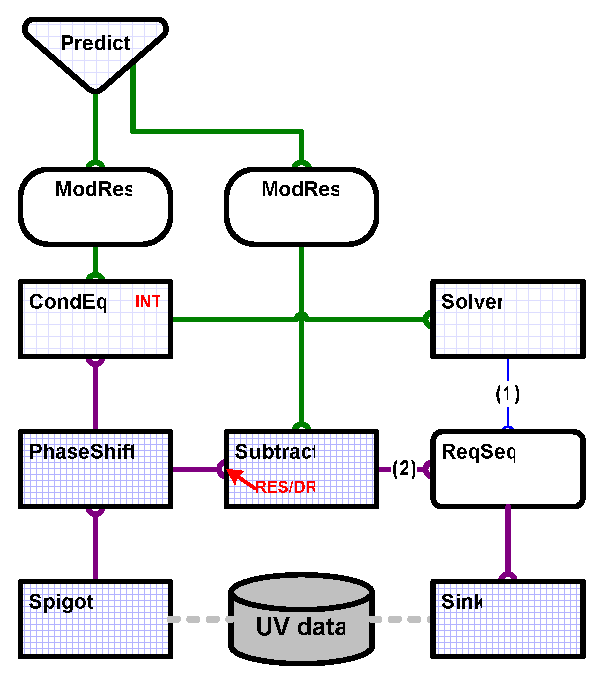
\includegraphics[width=.5\textwidth]{Figures/SolveMultiRes.eps}\\
  %% bb=38 554 327 811
  \end{center}
  \caption{\label{fig:resample}A multiple-resoulution tree employing
  auto-resampling}
  \end{figure}

\subsubsection{Implementation issues}

  For the time being, \qq{Node} only supports integral resamplings. In other
  words, the higher-resolution cells must be perfect tilings of the
  lower-resolution cells. A fail-result is generated otherwise. This keeps
  things simple, and avoids interpolation errors.\footnote{In the future, we
  may add support support arbitrary regridding if needed.} 

  This limitation is less serious than may appear. Resolutions are never chosen
  randomly -- from a tree designer's point of view, they are completely
  deterministic. Current facilities for resolution control (the \qq{ModRes}
  node mentioned below) only allow for integral resolutions. As for the
  original data resolution, it always comes in from the data access nodes
  (\qq{Sink} and \qq{Spigot}), which are tightly coupled: for each snippet of
  data, the \qq{Sink} issues a \Request\ with a \Cells\ corresponding to the
  data layout, while the corresponding \qq{Spigot} is then ready to return a
  \Result\ with the same cells. Thus, the tree designer can always define
  working resolutions for subtrees in terms of integral factors of the original
  data resolution.
  
  Upsampling currently uses linear interpolation. In the future, we may add
  support for more sophisticated resampling.

\subsection{Controlling the resolution}

  The \qq{ModRes} utility node may be used to change resolution mid-tree. A
  \qq{ModRes} always has a single child; upon receiving a \Request\ from its
  parent, it modifies its resolution up or down by a fixed factor (independent
  for each axis), as determined by its node state. The modified \Request\ is
  passed on to its child, and the child's \Result\ is returned directly to the
  parent.

  In the future, we envision an adaptive resolution reducer (ARR) node, which
  adaptively selects a minimum required resolution based on some
  application-specific considerations. These may include:

  \begin{itemize}
  
  \item For solving, the predict tree need only supply enough cells to
  constrain the solution. The minimum resolution can be determined by the
  \qq{Solver} node, and passed along in the \Request\ as a hint to any ARR nodes
  up the tree.
  
  \item For subtracting predicted sources, the cells need only be big enough
  to ensure linearity over a cell. 
  
  \end{itemize}
  
  Note also that the \qq{Identity} node, when configured with a ``Use Request''
  resampling strategy, becomes a {\em resolution coupler}, ensuring resampling
  all results to the requested resolution.

\subsection{How this applies to getResult()}
  \label{sec:getResult}

  Note that the \qq{getResult()} handler discussed above receives two crucial
  pieces of information: a vector of child results, and a \Cells\ (passed by
  ref). The \Cells\ parameter defines the expected result cells, and it is
  set up as follows:

  \begin{itemize}
  
  \item If auto-resampling is not enabled, or the node has no children, then
  this is simply the cells from the \Request. The resolutions of child results,
  if any, are not constrained.
  
  Note that most nodes' contracts specify that ``this node only deals with
  child results at the same resolution'' (this is true, e.g., for all
  \qq{Function} nodes), and leave it up to the tree designer to ensure it (i.e.
  by enabling auto-resampling where necessary). The node's behaviour when a
  contract is violated does not need to be defined (although one can reasonably
  expect an exception to be thrown, leading to a fail-result).

  \item If auto-resampling is enabled, then the resolutions of child results
  are constrained: they will all have the indicated \Cells\ (with the exception
  of resolution-free results, which have no cells). Most nodes are expected to
  return a result at the same resolution.

  \item If auto-resampling is enabled and all child results are
  resolution-free, then the \Cells\ ref is empty. In this case, most nodes'
  result will should be resolution-free as well. In the rare case where the
  node introduces its own time-frequency dependence (e.g. the \qq{UVW} node),
  it should get a \Cells\ from the request.

  \end{itemize}

\section{Function nodes}
\label{sec:Function}

  \qq{Function} is an important subclass of \qq{Node}, representing some
  function of its children's results. The main feature of \qq{Function} is an
  abstract \qq{evaluate()} method, which takes a vector of \Vells\ objects,
  computes some function over them, and returns a \Vells\ result.

  Remember that a \Vells\ is a an $N\times M$ matrix ($\bar{f}=\{f_{ij}\}$) of
  $\RR$ or $\CC$ values, representing a set of sampling or integrations of a
  function $f:\RR^2\rightarrow\RR$ or $f:\RR^2\rightarrow\CC$ over some cells.
  \Vells\ are organized into \VellSet{}s, containing the main value
  $\{f_{ij}\}$, plus an optional set of $K\times S$ $(S=1,2)$ perturbed values
  $\bar{f}_{sk} = \{f^{(sk)}_{ij}\}$, which correspond to $S$ sets of
  perturbations w.r.t. $K$ solvable parameters. A \VellSet\ will also contain
  $S$ vectors of the perturbations themselves, $\{\delta^{(s)}_k\}$.

  The \Result\ of child $l$ will contain $Q_l$ \VellSet{}s. Most of the time,
  $Q_l=1$; when $Q_l>1$, the result represents a multidimensional function
  $f:\RR^2\rightarrow\{\RR\mbox{ or }\CC\}^{Q_l}$. Note that each plane of such
  a function may have its own set of solvable parameters and perturbed values.
  We will use the notation $\bar{f}_{lq}$ to designate the main value for child
  $l$, plane $q$, and $\bar{f}^{(sk)}_{lq}$ to designate the corresponding
  perturbed value for parameter $k$ from set $s$.

  The \qq{evaluate()} method of a \qq{Function}-derived node implements some
  compound function of $L$ child \Vells\ defined over the same \Cells. We will
  designate this function as $F=F(\bar{f}_1,...,\bar{f}_L)$. The value of this
  function is a \Vells\ itself, $\bar{F} = \{F_{ij}\}$, also defined over the
  same \Cells. 

  The \qq{Function} class provides a \qq{getResult()} method that iterates over
  all \Vells\ in its child results, calls \qq{evaluate()} to compute $F$, and
  collect the resulting \Vells\ into an output \Result. The same operation is
  done for all perturbed values. Thus, the \qq{Function} class implements a
  basis for all nodes that calculate a compound function of their children.
  PSS4 includes an automatic code generator (documented elsewhere) that will
  generate a full C++ implementation of a \qq{Function}-derived node class,
  given a symbolic expression for the $F$ function. The kernel also provides a
  toolkit of \qq{Function}s that implement most primitive mathematical
  operations.

\subsection{Dealing with multiple planes}

  Note that an implementation of \qq{evaluate()} defines $F$ for a single set of
  \Vells. When child results contain multiple planes, \qq{Function} deals with
  it as follows:
  
  \begin{itemize}
  
  \item If all child results contain the same number of planes $Q$
  $(Q=Q_1=...=Q_L)$, the function $F$ is applied separately to each plane 
  $q=1...Q$.

  \item Child results with a different number of planes are supported in only
  one scenario: some results may have 1 plane, and some may have $Q>1$ planes,
  but $Q$ must be the same for all multi-planar results (a fail is generated if
  this condition is not met). Results with 1 plane are then artificially
  expanded to $Q$ planes by reusing the same \VellSet\ for all planes from 1 to
  $Q$. (This is roughly similar to scalar-vector operations in Glish.)

  \end{itemize}
  
\subsection{Dealing with perturbed values}

  Each plane (aka \VellSet) $q$ of result $l$ may contain a number of perturbed
  values. These are also evaluated. Note that the set of parameters (identified
  by spids) with respect to which the values are perturbed is not necessarily
  the same for each child result or plane, in fact, some planes or results may
  contain no perturbed values at all.
  
  To simplify the description here, let's remember that \qq{Function} deals
  with multiple result planes independently, on a plane-by-plane basis (see
  above). Hence, we'll assume we're dealing with only one plane, and $l$ child
  results for that plane. We'll also forget about multiple perturbation sets,
  since those are all dealt with in the same way. 

  \qq{Function} starts by figuring out all the spids present in the \VellSet{}s
  of the children. Thus, it ends up with a list of spids,
  $(\kappa_1,...,\kappa_n)$, which is simply the union of the spid sets from
  each child's \VellSet. For each spid $\kappa_i$, it then needs to compute the
  perturbed value of $F$ with respect to parameter $\kappa_i$
  $(\bar{F}^{(\kappa_i)})$, based on the perturbed \Vells\
  $(\bar{f}^{(k)})$ found in the child \VellSet{}s.

  This is done by calling \qq{evaluate()} $n$ times to compute
  $\bar{F}^{(\kappa_i)}$ for each $\kappa_i$, while selecting the input \Vells\
  from each child's result as follows. If spid $\kappa_i$ is present in the
  list of spids for  the \VellSet\ of child $l$, the perturbed value
  $\bar{f}^{(lk)}$ is used (where $k$ corresponds to spid $\kappa_i$).
  Otherwise, the main value $\bar{f}_l$ is used.

  If this seems complicated at first glance, remember that the end result is
  quite simple. A \qq{Function} node computes some function over its children's
  results. If the subtrees above the node contain solvable parameters, then
  perturbed values of that same function {\bf w.r.t. all the solvable
  parameters} must be computed as well, based on perturbed values returned by
  the children. Everything else follows from this simple requirement.

\subsection{Restrictions on child results}
   
  A \qq{Function} node imposes certain restrictions on the structure of its child
  results, which the tree designer should be aware of. If the results do not
  have the right layout, a fail is always generated.
  
  \begin{itemize}
  
  \item The first restriction has already been covered above -- all results must have
  the same number of planes, or must be a mix of $Q$ planes and single planes.
  \qq{Composer} and \qq{Selector} nodes should be placed appropriately to ensure
  this.
  
  \item The second restriction has also been mentioned -- all results must have
  the same \Cells. Auto-resampling may need to be enabled to ensure this. This
  implies that all \Vells\ in the results will have either the same $M\times N$
  shape, or will be scalars (i.e. no time-frequency dependence).
  
  \item The child results must be either all samplings or all integrations. The
  two types cannot be mixed in the same expression.

  \item The next restriction involves the values of the perturbations
  $(\delta_\kappa)$ themselves. When $F$ is evaluated over perturbed values for
  parameter $\kappa$, and these perturbed values appear in more than one
  \VellSet, the result is sensible only when the perturbation
  $\delta_\kappa$ is the same thoroughout. 

  \item Finally, if more than one perturbed value set is used (think
  double-differencing), \qq{Function} requires that all child results have the
  same number of sets, though any child may always return zero sets (no
  perturbed values at all).

  \end{itemize}
  
  Note that the last two restrictions are almost always met automatically,
  since the perturbations $\delta_\kappa$ are usually determined by the
  parameters (i.e. \qq{Parm} nodes) themselves. Single- or double-differencing
  is determined by the value of \qq{calc\_deriv} in the \Request, which is also
  the same for all children. You'd be hard-pressed to construct a tree that
  didn't meet these two restrictions. Nevertheless, it's something to keep in
  mind in case you see \qq{Function} nodes failing unexpectedly.

\subsection{Implementing evaluate(): Vells arithmetic}
  \label{sec:vells}

  The \qq{evaluate()} method is defined as follows:
  
  \begin{verbatim}  
  virtual Vells evaluate (const Request &req,
                          const LoShape &shape,
                          const std::vector<const Vells*> &args);
  \end{verbatim}
  
  The \qq{req} argument is simply the original \Request. \qq{shape} indicates
  the shape of the output \Vells\ (i.e. the shape of the result \Cells, see
  \ref{sec:getResult}). The last parameter is a vector of pointers to argument
  \Vells, which \qq{Function} sets up for each call so that the correct
  combination of main values and perturbed values is used. Note that the
  resulting \Vells\ is returned by value; this is a very fast operation, since
  \Vells\ utilizes copy-on-write for its contents.

  \begin{table}[th]
  \begin{center}\begin{tabular}{|p{.25\textwidth}p{.7\textwidth}|}
  
  \tablesubheading{2}{basic arithmetic:}\\
  \qq{-} & unary negation\\
  \qq{+ - * /} & standard binary arithmetic operators\\
  
  \tablesubheading{2}{in-place arithmetic:}\\
  \qq{+= -= *= /=} & arithmetic, modifies the left-hand \Vells\ in-place\\
  
  \tablesubheading{2}{unary functions, $\RR\rightarrow\RR$ and
                      $\CC\rightarrow\CC$:}\\
  \qq{exp() log() log10()} & $e^x$, $\ln{x}$, $\log{x}$\\
  \qq{sqr() sqrt()} & $x^2$, $\sqrt{x}$ \\
  \qq{pow2()}...\qq{pow8()} & $x^2...x^8$\\
  \qq{sin() cos() tan()} & sine, cosine, tangent \\
  \qq{sinh() cosh() tanh()} & hyperbolic sine, cosine, tangent \\
  \qq{conj()} & complex conjugate \\
  
  \tablesubheading{2}{unary functions, $\RR\rightarrow\RR$ only:}\\
  \qq{ceil()} & nearest integer $\ge x$\\
  \qq{floor()} & nearest integer $\le x$\\
  \qq{acos() asin() atan()} & arccosine, arcsine, arctangent \\
  
  \tablesubheading{2}{unary functions, $\RR\rightarrow\RR$ or 
                      $\CC\rightarrow\RR$:}\\
  \qq{abs() fabs()} & absolute value $|x|$ (both names are equivalent)\\
  \qq{norm()} & norm: $|x|^2$\\
  \qq{arg()} & argument of a complex number (the $\phi$ in $x=|x|e^{i\phi}$)\\
  \qq{real() imag()} & real and imaginary parts\\

  \tablesubheading{2}{array reductions:}\\ 
  
  \qq{min() max() mean() sum() product()} & these reduce the argument
  (presumbaly, an array \Vells) to a single scalar. Note that \qq{min()} and
  \qq{max()} are only defined for real arguments.\\

  \tablesubheading{2}{binary functions:}\\
  \qq{tocomplex()} & $x+iy$\\
  \qq{pow()} & $x^y$ \\
  \qq{atan2()} & $\arctan(y/x)$, also defined for $x=0$\\
  \qq{posdiff()} & angular difference: for two angles $x,y$ in the range
  $[-\pi,\pi]$, returns $x-y$ renormalized into $[-\pi,\pi]$ by adding $\pm2\pi$ as
  necessary.\\
  
  \hline
  \end{tabular}\end{center}
  
  {\em Note: some \Vells\ functions are defined for real arguments only.
  Applying them to a complex \Vells\ will result in a fail.}

  \caption{\label{table:vellsmath}Available \qq{Vells} operations}
  \end{table}

  Implementations can take advantage of {\em \Vells\ math}. \Vells\ is an
  intelligent wrapper for real or complex 2D arrays or scalars, with overloaded
  operators and functions for basic math and implicit conversion from scalar
  values to a \Vells. It provides automatic type promotion, and can also
  implictly ``expand'' a scalar to an array. For example, the doubled product
  of two \Vells\ \qq{a} and \qq{b} may be obtained simply by stating
  \qq{c=2*a*b}. This notation conveniently hides a lot of messy processing:
  real \Vells\ are automatically promoted to complex if the other argument is
  complex, scalars are expanded to arrays if the other argument is an array,
  and the operation is performed on an element-by-element basis.\footnote{An
  exception is thrown if two array \Vells\ have a different  shape. Note that
  having the same \Cells\ in all child results ensures the same shape for all
  \Vells.}  As another example, here's an actual implementation of
  \qq{evaluate()} for the \qq{Cos} node (computes cosine of child result):

  \begin{verbatim}
  Vells Cos::evaluate (const Request&,const LoShape &,
                       const vector<const Vells*>& args)
  {
    return cos(*(args[0]));
  }
  \end{verbatim}
  
  Table~\ref{table:vellsmath} lists all the primitive operators and functions 
  available with the \qq{Vells} class. Most of these operate on \qq{const}
  arguments and return a new \Vells\ object by value. The exception are 
  in-place operators (\qq{"+="} and friends), which modify a \qq{Vells} in
  place and return it as \qq{"Vells\&"} (these obviously require a
  non-\qq{const} argument). The C++ syntax allows one to freely combine
  primitive operations into complicated expressions, while the compiler takes
  care of creating and destroying intermediate \Vells\ objects as appropriate.

  \subsubsection{Copy-on-write specifics}

  Since \Vells\ employ copy-on-write, using \Vells\ math for complicated
  expressions incurs very little overhead in comparison to an ``optimized''
  implementation with explicit looping over array elements. The amount of
  messy coding saved, on the other hand, is huge. 
  
  Copy-on-write means that when one \Vells\ is assigned to or initialized from
  another \Vells, the two start off sharing the same data. This makes 
  copy/assignment operations very economical, since the underlying data array 
  is not copied. Any subsequent attempts to modify either \Vells\ will cause a
  true private copy of the data to be made. Thus, copying of data arrays is
  deferred until it is actually needed (which may be never). 

  Consider, for example, an implementation of \qq{Add:evaluate()}. The \qq{Add}
  node adds the results of any number of children:

  \begin{verbatim}  
  Vells Add::evaluate (const Request&, const LoShape&,
                       const vector<const Vells*>& args)
  {
    if( args.empty() )
      return Vells(0.);
    Vells result(*args[0],DMI::READONLY);
    for( uint i=1; i<args.size(); i++ )
      result += *(args[i]);
    return result;
  }
  \end{verbatim}  
  
  The \qq{result} \Vells\ is initialized from the first argument \Vells, and
  shares data with it. As soon as the second argument is added in, a private 
  copy of \qq{result}'s data is implicitly created. If, however, only one
  argument is passed in to begin with, the \qq{result} will still share data
  with it when returned.

%  The \MeqServer\ object provides an interface to the MeqTree kernel. It 
  
  
